\section{Methodology}
\label{sec:methodology}



We propose \emph{\textbf{Skill} \textbf{S}elf-\textbf{P}lay} (\textbf{Skill-SP}), a training-time framework that transforms generic self-play into a proactive curriculum-construction process (Figure~\ref{fig:method}). At each iteration, Skill-SP orchestrates the joint optimization of a proposer policy $\pi_\text{propose}$ and a solver policy $\pi_\text{solve}$, alongside a skill controller managing an evolving library $\gS$. Guided by routed skills, the proposer is updated to synthesize valid tasks at the solver's learning frontier, while the solver is optimized on the resulting verified curriculum. Concurrently, the controller distills execution feedback to update the library, driving a continuous co-evolutionary loop that yields progressively more informative challenges.


\begin{figure}[t]
    \centering
    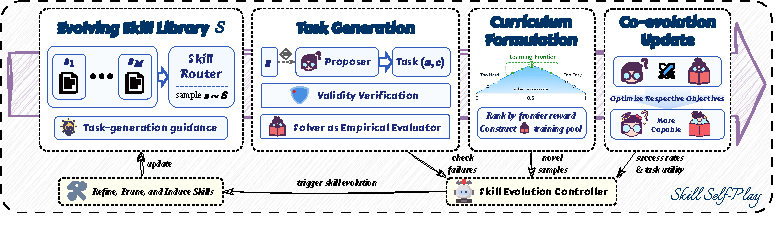
\includegraphics[width=0.98\linewidth]{figures/method.pdf} 
    \vspace{-0.5em}
    \caption{\textbf{Overview of Skill Self-Play.} An evolving skill library routes task-generation guidance to the proposer, which generates candidate tasks that undergo validity verification. Valid candidates are ranked by frontier reward to construct the solver curriculum. The resulting signals drive co-evolutionary proposer and solver updates, while validation failures, novel samples, and task-level statistics trigger skill refinement, pruning, and induction, distilling training feedback into reusable skills for subsequent task generation.}
    \label{fig:method}
\end{figure}



\subsection{Skill Self-Play Objective}
\label{sec:osp_objective}

We formalize a verifiable agent task as a tuple $(\vx,\vc)$, where $\vx$ is the standard prompt visible to the solver, and $\vc$ is a hidden, machine-readable verification contract (e.g., unit tests, reference answers) evaluated exclusively by the environment. Given a solver's response $\vy$, the environment returns a verification reward $\mathcal{R}_\text{solve}(\vx,\vy,\vc) \in [0,1]$.

A standard self-play loop trains the proposer to generate challenging tasks and the solver to resolve them. For a generated task instance $(\vx,\vc)$, the solver's expected success rate is defined as:
\begin{equation}
v_\text{solve}(\vx,\vc;\pi_\text{solve})
=
\mathbb{E}_{\vy \sim \pi_\text{solve}(\cdot \mid \vx)}
\left[
    \mathcal{R}_\text{solve}(\vx,\vy,\vc)
\right].
\label{eq:osp_empirical_success}
\end{equation}
To drive continuous improvement, a natural objective for the proposer is to target the solver's learning frontier via a medium-difficulty score, formulated as $1 - 2|v_\text{solve} - 0.5|$. However, optimizing the proposer solely toward this metric frequently invites \emph{reward hacking}, where the proposer synthesizes ill-posed or unsolvable contracts to fabricate artificial difficulty.
To prevent this, Skill-SP formalizes task generation via a \emph{gated curriculum reward}. We introduce a binary task quality filter that retains only candidates with structurally sound contracts, thereby explicitly gating the proposer's reward:
\begin{equation}
\gR_\text{propose}(\vx,\vc;\pi_\text{solve})
=
\mathbb{1}_{\{(\vx,\vc) \text{ is valid}\}}
\cdot
\big(
    1 - 2
    \Big|
        v_\text{solve}(\vx,\vc;\pi_\text{solve})
        - \frac{1}{2}
    \Big|
\big),
\label{eq:frontier_score}
\end{equation}
where the indicator $\mathbb{1}_{\{(\vx,\vc) \text{ is valid}\}}$ represents this binary filter, which is further detailed in Eq.~\ref{eq:valid-task-indicator} of Section~\ref{sec:proposer_optimization}.

To proactively guide task generation, Skill-SP introduces an evolving skill library $\gS$. Task synthesis is conditioned on a sampled skill $\vs \sim \gS$, which equips the proposer with reusable structural priors and programmatic validators. Consequently, Skill-SP can be formulated as a bi-level optimization problem. The outer objective jointly optimizes the skill library $\gS$ and the proposer $\pi_\text{propose}$ to synthesize valid, frontier-targeted tasks, subject to an inner objective where the solver maximizes its execution success on these tasks:
\begin{equation}
\begin{aligned}
    \max_{\pi_\text{propose}, \gS} \quad
    & \mathbb{E}_{\vs \sim \gS,\;(\vx,\vc)\sim \pi_\text{propose}(\cdot\mid\vs)}
    \left[\gR_\text{propose}(\vx,\vc;\pi^*_\text{solve})\right] \\
    \text{s.t.} \quad
    &
    \pi^*_\text{solve}
    =
    \arg\max_{\pi}
    \mathbb{E}_{
        \vs\sim \gS,\; (\vx,\vc)\sim\pi_\text{propose}(\cdot\mid\vs),\;
        \vy\sim\pi(\cdot\mid\vx)
    }
    \left[
        \mathcal{R}_\text{solve}(\vx,\vy,\vc)
    \right].
\end{aligned}
\label{eq:bilevel_optimization}
\end{equation}
To orchestrate this high-fidelity curriculum loop, the subsequent sections detail the policy optimization of the proposer and the solver, alongside the dynamic evolution of the skill library $\gS$.



\subsection{Proposer Optimization via Skill-Conditioned Generation}
\label{sec:proposer_optimization}

To operationalize the outer objective (Eq.~\ref{eq:bilevel_optimization}), the proposer must continuously synthesize valid, frontier-targeted tasks. We structure this process into three stages: skill-conditioned generation to inject structural priors, rigorous verification to ensure task validity, and policy optimization to drive curriculum evolution.

\textbf{Skill-Conditioned Generation.}
A skill $\vs \in \gS$ serves as a structural interface defined by the tuple $\vs = \langle m, r, h, e, \nu, \sigma \rangle$. Here, $m$ denotes routing metadata; $r$, $h$, and $e$ provide procedural rules, generation hints, and few-shot examples to contextually condition the proposer; $\nu$ specifies executable validators; and $\sigma$ tracks historical usage statistics. During generation, we dynamically sample a skill $\vs \sim \gS$ based on $\sigma$, balancing the exploitation of high-yield skills with an exploration bonus for under-tested ones (detailed in Appendix~\ref{app:skill_routing}). The proposer then synthesizes candidates via a \emph{skill stream} $(\vx,\vc) \sim \pi_\text{propose}(\cdot \mid \vs)$, which injects strong structural priors. To continuously chart novel task spaces and prevent mode collapse, this is complemented by an open-ended \emph{exploration stream} $(\vx,\vc) \sim \pi_\text{propose}(\cdot \mid \varnothing)$ without skill constraints.

\textbf{Validity Verification.}
The binary task quality filter $\mathbb{1}_{\{(\vx,\vc) \text{ is valid}\}}$ gating the proposer reward (Eq.~\ref{eq:frontier_score}) enforces rigorous structural and logical checks. For tasks generated via the skill stream, this valid event is defined as the intersection of three conditions:
\begin{equation}\label{eq:valid-task-indicator}
    \big\{(\vx,\vc) \text{ is valid}\big\} = \big\{\text{schema compliant}\big\} \cap \big\{\text{contract valid}\big\} \cap \big\{\text{probe consistent}\big\}.
\end{equation}
Here, the first condition ensures global schema compliance; the second applies validators defined in $\vs$ to filter ill-posed contracts; and the third verifies \emph{probe consistency}. Specifically, this consistency requires that $K$ rollouts drawn from the current solver $\pi_\text{solve}(\cdot \mid \vx)$ yield a unique majority answer matching the proposer-defined reference in $\vc$. For the exploration stream, the valid event omits this skill-specific validation.

\textbf{Policy Update.}
At each training iteration $t$, we fix the current solver $\pi_{\text{solve}}^{(t)}$ to serve as an empirical evaluator. For each generated candidate, we compute the gated reward $\gR_\text{propose}$ by combining its validity mask $\mathbb{1}_{\{(\vx,\vc) \text{ is valid}\}}$ with the empirical success rate $v_\text{solve}(\vx,\vc;\pi_{\text{solve}}^{(t)})$, efficiently estimated by reusing the $K$ verification rollouts. The proposer policy $\pi_{\text{propose}}^{(t)}$ is then updated via Group Relative Policy Optimization (GRPO)~\citep{shao2024deepseekmath} to maximize the expected reward:
\begin{equation}
\mathcal{J}_{\text{propose}}(\pi)
=
\mathbb{E}_{\vs \sim \gS, \; (\vx,\vc) \sim \pi(\cdot \mid \vs)}
\left[
\gR_{\text{propose}}
(\vx,\vc;\pi_{\text{solve}}^{(t)})
\right].
\label{eq:proposer_rl_objective}
\end{equation}
Optimizing this objective yields the next-iteration proposer $\pi_{\text{propose}}^{(t+1)}$, ensuring that as the solver evolves, the proposer dynamically tracks its shifting learning frontier to continuously synthesize challenging, reliable tasks.



\subsection{Solver Optimization via Dynamic Curriculum Construction}
\label{sec:solver_optimization}

To operationalize the inner objective (Eq.~\ref{eq:bilevel_optimization}), the solver is optimized on a dynamic curriculum that systematically advances its capabilities. We construct this high-quality training pool by selecting the most challenging, frontier-targeted tasks from both generation streams.

\textbf{Curriculum Construction.}
Let $\mathcal{T}_{\text{skill}}^{(t)}$ and $\mathcal{T}_{\text{explore}}^{(t)}$ denote the sets of strictly valid candidates $(\vx,\vc)$ synthesized by the skill and exploration streams, respectively. To form the final training pool $\mathcal{D}^{(t)}$ of size $M$, we rank these candidates by their proposer reward $\gR_{\text{propose}}(\vx,\vc;\pi_{\text{solve}}^{(t)})$, effectively pinpointing the solver's learning frontier, and select the top-scoring tasks according to a blending ratio $\alpha \in (0,1)$:
\begin{equation}
    \mathcal{D}^{(t)}
    =
    \mathrm{Top}_{\alpha M} \! \left(\mathcal{T}_{\text{skill}}^{(t)}; \gR_\text{propose}\right)
    \; \cup \;
    \mathrm{Top}_{(1-\alpha) M} \! \left(\mathcal{T}_{\text{explore}}^{(t)}; \gR_\text{propose}\right).
    \label{eq:mixed_pool}
\end{equation}

\textbf{Policy Update.}
Using the constructed curriculum $\mathcal{D}^{(t)}$, the solver policy $\pi_{\text{solve}}^{(t)}$ is updated via GRPO to maximize the environment verification reward:
\begin{equation}
\mathcal{J}_{\text{solve}}(\pi)
=
\mathbb{E}_{
(\vx,\vc)\sim\mathcal{D}^{(t)},\;
\vy\sim\pi(\cdot\mid\vx)
}
\left[
\mathcal{R}_{\text{solve}}(\vx,\vy,\vc)
\right].
\label{eq:solver_rl_objective}
\end{equation}
Optimizing this objective yields the next-iteration solver $\pi_{\text{solve}}^{(t+1)}$.



\subsection{Continuous Evolution of the Skill Library}
\label{sec:skill_evolution}

To prevent curriculum stagnation, the skill library $\gS^{(t)}$ dynamically co-evolves with the proposer and solver policies at each iteration $t$. This evolution comprises three operations: refining existing skills, pruning obsolete ones, and inducing novel structural priors from open-ended exploration.

\textbf{Skill Refinement.}
Using generation feedback, Skill-SP updates the tracking statistics $\sigma$ of each sampled skill to modulate future routing (Appendix~\ref{app:skill_routing}). Concurrently, it analyzes execution trajectories from invalid generation attempts to diagnose systematic failures and automatically refine the core content of the skills, maintaining the library as a robust repository of structural priors.

\textbf{Skill Pruning.}
To maximize sample efficiency, the active library undergoes periodic pruning. By monitoring $\sigma$, Skill-SP identifies a pruning set $\mathcal{S}_{\text{prune}}^{(t)}$ of saturated skills that consistently yield trivial tasks, indicated by an expected frontier reward falling below a threshold $\gamma_{\text{prune}}$:
\begin{equation}
    \mathcal{S}_{\text{prune}}^{(t)} = \left\{ \vs \in \gS^{(t)} \;\middle|\; \mathbb{E}_{(\vx,\vc)\sim\pi_{\text{propose}}^{(t)}(\cdot\mid\vs)} \big[ \gR_{\text{propose}}(\vx,\vc;\pi_{\text{solve}}^{(t)}) \big] < \gamma_{\text{prune}} \right\}.
\end{equation}
Archiving $\mathcal{S}_{\text{prune}}^{(t)}$ conserves the generation budget and keeps the proposer focused on the learning frontier.

\textbf{Skill Induction and Update.}
To systematically expand the curriculum, Skill-SP extracts an induction set $\mathcal{T}^{(t)}_{\text{induce}}$ of novel candidates from the exploration stream, conditioned on a minimum frontier reward threshold $\gamma_{\text{induce}}$:
\begin{equation}
    \mathcal{T}^{(t)}_{\text{induce}} = \left\{ (\vx,\vc) \in \mathcal{T}_{\text{explore}}^{(t)} \;\middle|\; \gR_{\text{propose}}(\vx,\vc;\pi_{\text{solve}}^{(t)}) \ge \gamma_{\text{induce}} \right\}.
\end{equation}
Skill-SP then leverages the skill controller $\pi_{\text{control}}$, instantiated by the initial base policy, to abstract the underlying task patterns within $\mathcal{T}^{(t)}_{\text{induce}}$ into candidate packages. These are systematically filtered for structural integrity and semantic novelty against the current library to yield the newly induced skills $\gS_{\text{new}}^{(t)}$:
\begin{equation}
    \gS_{\text{new}}^{(t)} = \big\{ \vs \sim \pi_{\text{control}}( \cdot | \mathcal{T}^{(t)}_{\text{induce}}) \;\big|\; \operatorname{Integrity}(\vs) \wedge \operatorname{Novelty}(\vs, \gS^{(t)}) \big\},
\end{equation}
where $\operatorname{Integrity}(\vs)$ checks package completeness, and $\operatorname{Novelty}(\vs,\gS^{(t)})$ rejects candidates duplicating existing skills by thresholding lexical similarity.
The active library is subsequently updated via $\gS^{(t+1)} = (\gS^{(t)} \setminus \mathcal{S}_{\text{prune}}^{(t)}) \cup \gS_{\text{new}}^{(t)}$. This mechanism distills successful open-ended exploration into reusable structural priors, driving an ever-expanding curriculum. Algorithm~\ref{alg:skill_sp_overview} summarizes the resulting training loop.



\begin{algorithm}[t]
    \caption{{Skill Self-Play} (Skill-SP)}
    \label{alg:skill_sp_overview}
    \KwIn{Initial proposer $\pi_\text{propose}^{(0)}$, solver
    $\pi_\text{solve}^{(0)}$, skill library $\gS^{(0)}$, and number of
    self-play iterations $T$.}
    \KwOut{Trained solver $\pi_\text{solve}^{(T)}$.}

    \ForEach{self-play iteration $t$}{
        Sample $\vs\sim\gS^{(t)}$ using skill statistics; generate candidates with
        $\pi_\text{propose}^{(t)}(\cdot\mid\vs)$ and
        $\pi_\text{propose}^{(t)}(\cdot\mid\varnothing)$\;

        Verify candidates and compute $\gR_\text{propose}$; retain valid candidates for the solver curriculum\;

        Rank valid candidates by $\gR_\text{propose}$ to build the mixed
        frontier curriculum $\mathcal{D}^{(t)}$\;

        Update $\pi_\text{propose}^{(t)}\!\rightarrow\!
        \pi_\text{propose}^{(t+1)}$ using $\mathcal{J}_\text{propose}$, and
        $\pi_\text{solve}^{(t)}\!\rightarrow\!\pi_\text{solve}^{(t+1)}$
        on $\mathcal{D}^{(t)}$ using $\mathcal{J}_\text{solve}$\;

        Evolve the skill library by updating skill statistics, refining existing skills from failure traces, inducing new skills $\gS_{\text{new}}^{(t)}$ from
        induction candidates $\mathcal{T}_{\text{induce}}^{(t)}$, and pruning obsolete skills
        $\mathcal{S}_{\text{prune}}^{(t)}$:
        $\gS^{(t+1)}\gets
        (\gS^{(t)}\setminus\mathcal{S}_{\text{prune}}^{(t)})\cup
        \gS_{\text{new}}^{(t)}$\;
    }
    \Return{$\pi_\text{solve}^{(T)}$}\;
\end{algorithm}